\documentclass[12pt, a4paper]{article}

\usepackage[utf8]{inputenc}
\usepackage[hmargin=2cm,vmargin=2cm]{geometry}
\usepackage[brazil]{babel}
\usepackage{graphicx}
\usepackage{amsmath}
\usepackage{steinmetz}
\usepackage{float}

\title{Relatório 1\\Exercício Prático \textit{PSpice}}
\author{Gustavo Ciotto Pinton - 117136}
\date{Abril 2013}

\begin{document}

%    \maketitle
    {\large
    \centerline{Exercício Prático 1}
    \centerline{Gustavo Ciotto Pinton 117136}
    }
    \section*{Questões}
    
    \begin{enumerate}
    
        \item
            O circuito utilizado na questão seguinte está representado na figura logo abaixo, gerada através do \textit{software} PSpice.
            
            \begin{figure}[h!] 
                \centering
                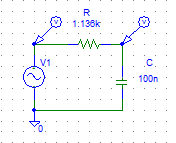
\includegraphics[width=0.250\textwidth]{circ1}
                \caption{circuito RC passa-baixos.}        
                \label{circ1}
            \end{figure}
    
    
        \item A frequência de corte teórica para o circuito da figura~\ref{circ1} é calculada através das seguintes expressões:
            \begin{equation} \label{eq:RCbaixo}
            T(jw)=\frac{V_c}{V_{in}}=\frac{Z_c}{R+Z_c}=\frac{\frac{1}{jwC}}{R+\frac{1}{jwC}}=\frac{1}{1+jwRC}=\frac{1}{1+j\frac{w}{w_c}}
            \end{equation}
            Portanto, para circuitos passa baixos, a equação~\ref{eq:RCbaixo} define a frequência de corte por: 
            
            \begin{equation}
            w_c = \frac{1}{RC}
            \end{equation}
            
            ou
            
            \begin{equation} \label{eq:FreqRC}
            f_c = \frac{1}{2 \pi RC}
            \end{equation}
            
            Utilizando a equação~\ref{eq:FreqRC} para os valores da figura~\ref{circ1}, isto é, \( R = 1.136k\Omega\) e \(C = 100nF\), obtém-se \(f_c = \frac{1}{2\pi*1136*10^{-7}}=1.4kHz\).\\
            Se o módulo da função \(T(jw)\) for calculado, então é possível determinar a amplitude da tensão de saída no capacitor. Desta maneira, através da equação~\ref{eq:RCbaixo}, tem-se:
            
            \begin{equation} \label{eq:amp1}
            \left|T(jw)\right| = \left|\frac{V_c}{V_{in}}\right| = \left|\frac{1}{1+j\frac{w}{w_c}}\right| = \frac{1}{\sqrt{1+(\frac{f}{f_c})^2}}
            \end{equation}
            
            De~\ref{eq:amp1}, obtém-se:
            \begin{equation} \label{eq:ampVc}
            \left|V_c\right| = \frac{1}{\sqrt{1+(\frac{f}{f_c})^2}}*\left|V_{in}\right|
            \end{equation}
            
            Se \(\left|V_{in}\right| = 1V\), \(f=1kHz\) e \(f_c=1.4kHz\), então pela equação~\ref{eq:ampVc}, \(\left|V_{c}\right| = 0.81V\).
            
            Da mesma maneira, é possível obter a diferença de fases entre as ondas de entrada e saída, através de \ref{eq:RCbaixo}:
            
            \begin{equation} \label{eq:fase1}
            \phase{T(jw)} = -\arctan{\left(\frac{f}{f_c}\right)}
            \end{equation}
            
            Se \(f=1kHz\) e \(f_c=1.4kHz\), então pela equação~\ref{eq:fase1}, \(\phase{T(jw)} = \theta = -35,5º\). \\
            
            Os gráficos obtidos da simulação do experimento foram:
            
            \begin{figure}[h!] 
                \centering
                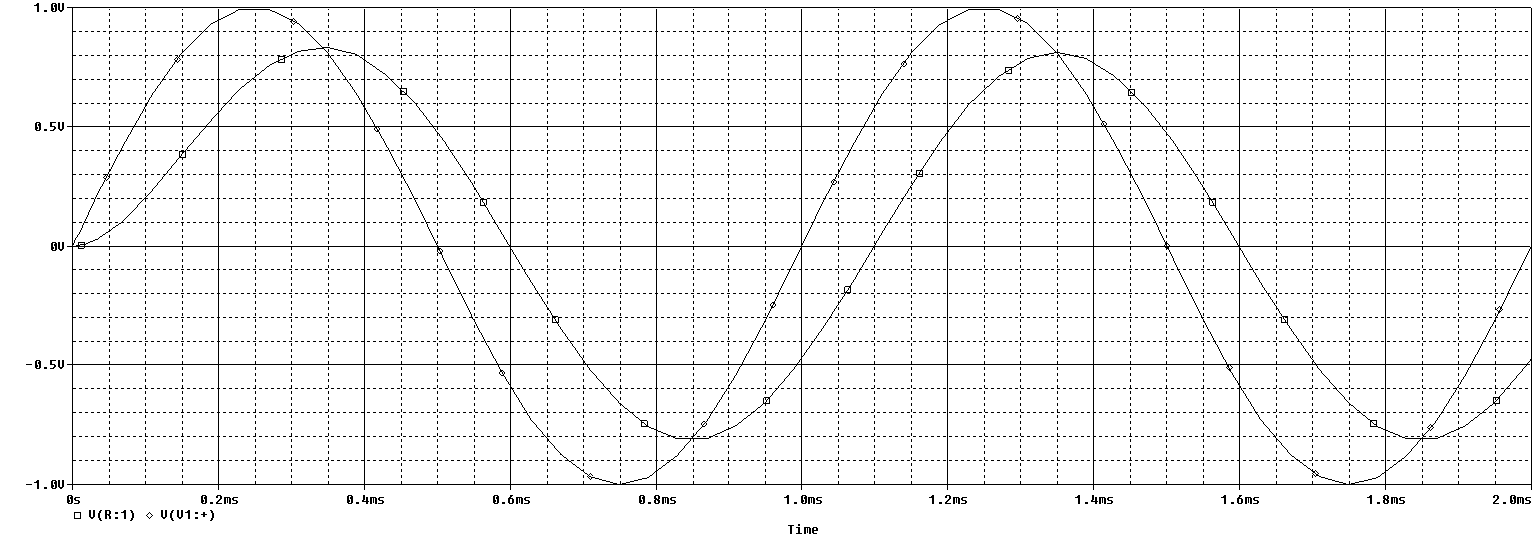
\includegraphics[width=1\textwidth]{waves1}
                \caption{ondas de entrada e saída.}        
                \label{waves1}
            \end{figure}
            
            \begin{figure}[h!] 
                \centering
                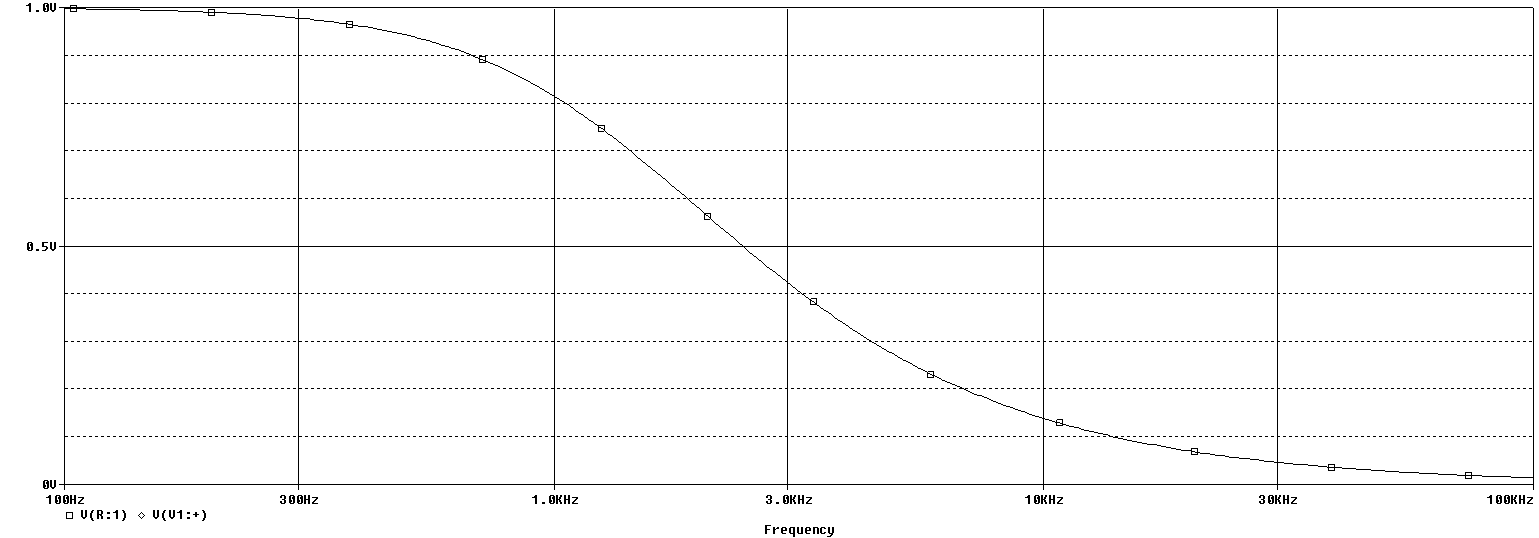
\includegraphics[width=1\textwidth]{waves2}
                \caption{tensão de sáida em função da frequência}        
                \label{waves2}
            \end{figure}
            
            Portanto, analisando as figuras \ref{waves1} e \ref{waves2}, é possível concluir que os resultados teóricos encontrados adequam-se aos dados obtidos através da simulação. Em outras palavras, vê-se que a amplitude da onda de saída, representada na figura \ref{waves1}, é de fato próximo do valor de 0.81V, e que ela está avançada em relação à onda de entrada em um ângulo de aproximadamente 35.5º. Da figura~\ref{waves2}, obtem-se que o valor de 0.5V é atingido quando a frequência é próxima de \(f = 1.4kHz\), o que já era esperado.
            
            \item O esquema do amplificador inversor está respresentado na figura logo abaixo:
            
            \begin{figure}[h!] 
                \centering
                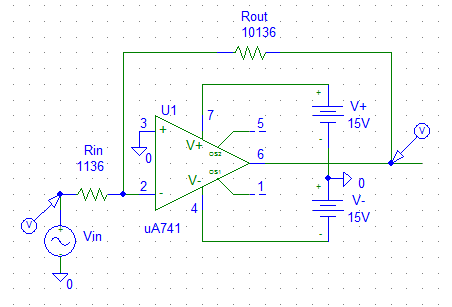
\includegraphics[width=0.35\textwidth]{circ3}
                \caption{amplificador inversor.}        
                \label{circ3}
            \end{figure}
            
            Na figura~\ref{circ3}, a amplitude da fonte de entrada é \(\left|V_{in}\right| = 1V\) e sua frequência é \(f=1kHz\).
            O ganho esperado para um amplificador ideal, com ganho infinito, segue a expressão:
            \begin{equation} \label{eq:ganho}
            \frac{V_{out}}{V_{in}} = - \frac{R_{out}}{R_{in}}
            \end{equation}
            
            Para \(R_{in}=1.136k\Omega\) e \(R_{out}=10.136k\Omega\), a expressão~\ref{eq:ganho} torna-se 
            \begin{equation} \label{eq:ganhoVa}
            \frac{V_{out}}{V_{in}} = - \frac{R_{out}}{R_{in}} = - \frac{10.136}{1.136} = -8.922
            \end{equation}
            e a amplitude da tensão de saída esperada, \(\left|V_{out}\right|\), é igual a \(8.922V\).\\
            Usando a ferramenta \textit{Analysis} do \textit{PSpice}, obtém-se o gráfico de transientes da figura~\ref{waves3}, logo abaixo.
            
            \begin{figure}[h!] 
                \centering
                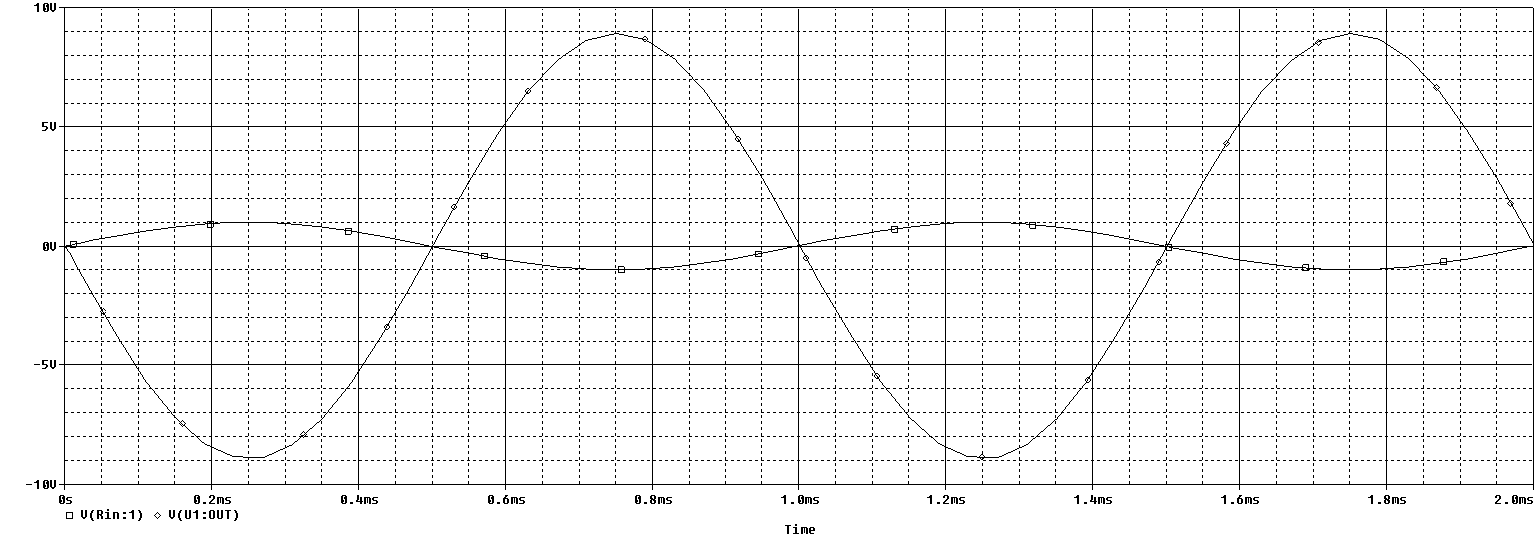
\includegraphics[width=1\textwidth]{waves3}
                \caption{ondas de entrada e saída.}        
                \label{waves3}
            \end{figure}
            
            Nesta figura, observa-se que quando a onda de entrada atinge um pico positivo, a onda de saída atinge um negativo, e vice-versa, justificando a função inversora do circuito. Observa-se também que a amplitude máxima da saída está de acordo com aquela teórica encontrada na expressão~\ref{eq:ganhoVa}, cujo valor aproxima-se de \(9V\) (\(\approx 8.922V\)).
            
            \item O circuito amplificador integrador utilizado está representado na figura~\ref{circ4}.
             
            \begin{figure}[H] 
                \centering
                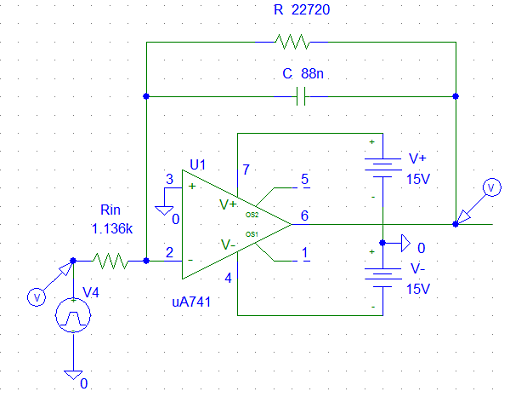
\includegraphics[width=0.35\textwidth]{circ4}
                \caption{circuito amplificador integrador.}        
                \label{circ4}
            \end{figure} 
            
            A equação que caracteriza o integrador amplificador RC é:
            
            \begin{equation} \label{eq:integRC}
                V_o = -\frac{1}{R_{in}C}\int_0^{t}V_{in}dt + V_0(t_0)
            \end{equation}
            
            Neste exercício, supomos o capacitor inicialmente descarregado, ou seja, \(V_0(t_0)=0\). \\ Através da expressão~\ref{eq:integRC}, pode-se calcular o valor da capacitância, isolando o termo C e integrando somente a parte da onda de entrada em que a amplitude é positiva e igual a \(V_{in} = 1V\). Deste modo, os limites da integral são definidos de 0 até metade da onda completa, isto é, \(\frac{T}{2}\). Sendo assim:
            
            \[C = \frac{1}{R_{in}V_0}\frac{T}{2} = \frac{1}{R_{in}V_0}\frac{1}{2f}\]
            
            Substituindo todos os valores (\(R_{in}=1136\Omega\) e \(V_0=5V\)), obtém-se \(C=88nF\). A partir de C, se \(RC=2ms\), então \(R = 22.72k\Omega\).
            
            As ondas de saída geradas por esse circuito estão representadas a figura~\ref{waves4}, logo abaixo. \\
            
            \begin{figure}[H] 
                \centering
                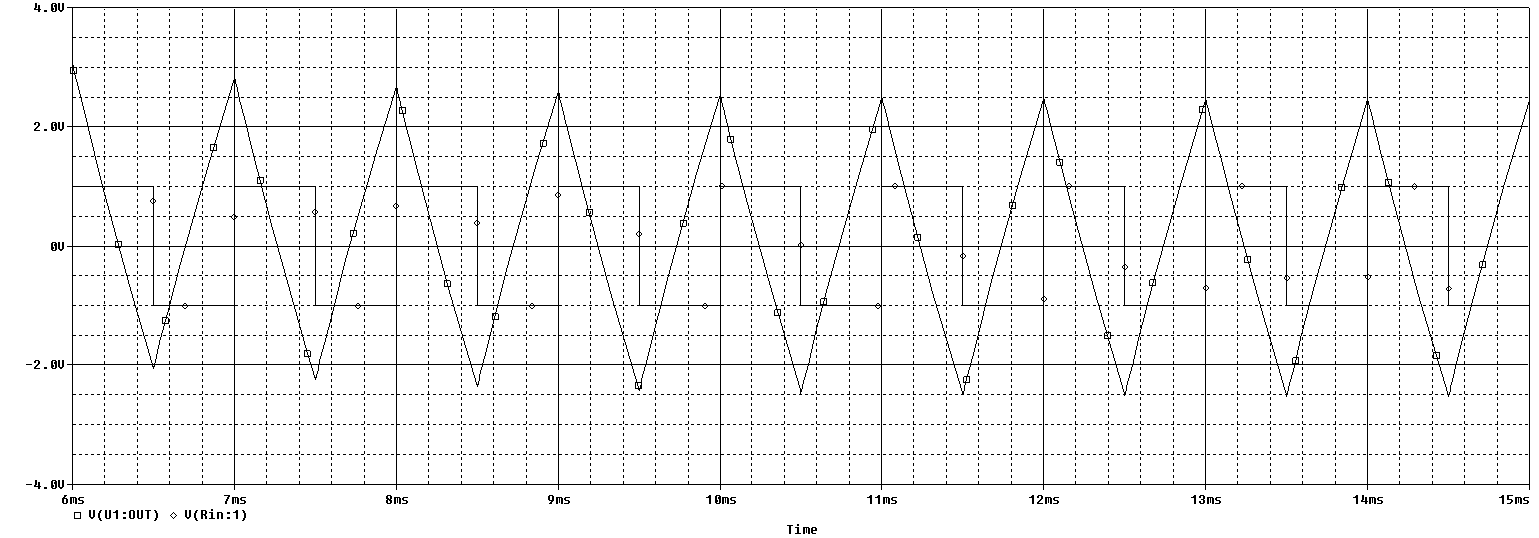
\includegraphics[width=1\textwidth]{waves4}
                \caption{ondas de entrada e saída.}        
                \label{waves4}
            \end{figure}
            
            A figura~\ref{waves4} segue o que calculamos na teoria, através da equação~\ref{eq:integRC}. Anteriormente, calculamos os valores das componentes para que a tensão pico-a-pico fosse de 5V, porém, no gráfico, obteve-se uma tensão pico-a-pico bem próxima de \(6V\). Esta pequena diferença ocorre devido a outra resistência utilizada, que não foi incluida na conta da equação~\ref{eq:integRC}. Observa-se também que, como esperado, o circuito comporta-se como inversor: quando a onda de entrada tem amplitude positiva, a inclinação da onda de saída é negativa e vice-versa.
            
            \item
            
            Configurando o \textit{AC Sweep} para simular frequências de \(1Hz\) até \(100kHz\), obtém-se o gráfico da figura \ref{waves5}.
            
            \begin{figure}[h!] 
                \centering
                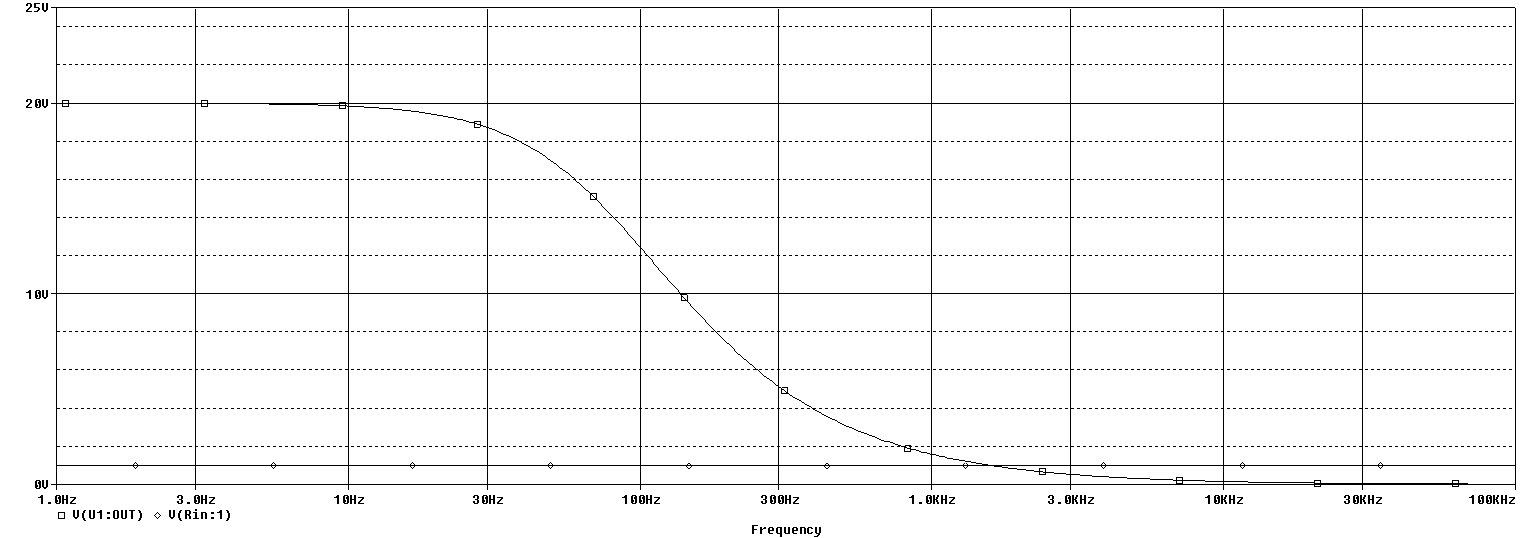
\includegraphics[width=1\textwidth]{waves5}
                \caption{análise de frequência do circuito da figura~\ref{circ4}.}        
                \label{waves5}
            \end{figure}
            
            Algumas expressões que nos ajudarão a entender e a avaliar a qualidade deste gráfico serão apresentados em seguida. Vale lembrar que, para este item, a fonte de ondas quadradas foi substituída por uma senoidal.\\
            
            A impedância equivalente da associação em paralelo de \(R\) e \(C\) é calculada por 
            \begin{equation} \label{eq:impeq}
            Z_{eq}=\frac{RX_c}{R+X_c}=\frac{R}{RCs+1}
            \end{equation} 
            em que \(s=jw\).
            O ganho de tensão é calculado usando as equações~\ref{eq:ganho} e \ref{eq:impeq} e é dada por:
            \begin{equation} \label{eq:ganho4}
            T(s)=\frac{V_{out}}{V_{in}} = -\frac{R}{R_{in}}\frac{1}{RCs+1}
            \end{equation}
            
            em que a amplitude é
            \begin{equation} \label{eq:amp4}
            \left|T(jw)\right|= \left|\frac{V_{out}}{V_{in}}\right| = \frac{R}{R_{in}}\frac{1}{\sqrt{(RCw)^2+1}}
            \end{equation}
            
            
%            A aproximação da equação~\ref{eq:amp4} pode ser feita porque assume-se que %o fator 1 é descartado devido as altas resistências \(R\) e \(R_{in}\). Sendo assim, se %\(V_{in} = 1V\), a amplitude da saída igual \(V_{out}=5V\) e \(f=1kHz\), então, de %acordo com a equação~\ref{eq:amp4}, \(C=28.02nF\). É possível calcular o valor do %resistor \(R\) para que a constante de tempo seja \(2ms\). Se \(RC=2ms\), então \(R = %71.38k\Omega\).\\    
            
            Vamos calcular alguns valores importantes e comparar os resultados entre teoria e o gráfico obtido. De acordo com a equação~\ref{eq:ganho4}, podemos obter a expressão da frequência de corte do circuito:
            
            \begin{equation} \label{eq:corte5}              
            f_c = \frac{1}{2 \pi RC}
            \end{equation}
            
            Substituindo os valores de R e C, calculados no item anterior, isto é, \(C=88nF\) e \(R=22.72k\Omega\), na expressão anterior e na \ref{eq:amp4}, tem-se, respectivamente: \[f_c=79.6Hz\] e \[\left|T_c\right| = \frac{R}{R_{in}}\frac{1}{\sqrt{2}}= 14.14V \]
            
            Os valores teóricos encontrados correspondem a aqueles presentes no gráfico, ou seja, para um valor de tensão de saída de aproximadamente de \(14.14V\), a frequência é também próxima de \(f_c = 79.6Hz\), sendo que especificamente neste ponto, a função de transferência adquire o comportamento decrescente máximo. 
            
    \end{enumerate}

\end{document}